\section{O que já foi feito}

\subsection{Lista de requisitos funcionais e não funcionais}
\subsubsection{Lista de requisitos funcionais}
\renewcommand{\arraystretch}{1.3}
\begin{center} % Centralizar a tabela
\begin{longtable}{|c|p{9cm}|c|} % Reduzi a largura da coluna de descrição
    \hline
    \textbf{Referência} & \textbf{Descrição} & \textbf{Prioridade} \\
    \hline
    RF01 & Eu, como utilizador, quero criar uma conta para poder aceder à plataforma e usufruir dos serviços. & Alta \\
    \hline
    RF02 & Eu, como utilizador, quero fazer \textit{login} para poder aceder à minha conta e \textit{gerenciar} os meus dados. & Alta \\
    \hline
    RF03 & Eu, como utilizador, quero criar e editar \textit{skills} para poder associá-las a talentos e melhorar a minha pesquisa e gestão de profissionais. & Alta \\
    \hline
    RF04 & Eu, como utilizador, quero apagar uma \textit{skill} apenas se ela não estiver associada a nenhum talento para garantir a consistência dos dados. & Alta \\
    \hline
    RF05 & Eu, como utilizador, quero pesquisar talentos por uma combinação de \textit{skills} para encontrar o profissional adequado para as necessidades de um cliente ou projeto. & Alta \\
    \hline
    RF06 & Eu, como utilizador, quero gerar um relatório com o preço médio mensal por categoria de talento e por país para analisar as tendências salariais e tomar decisões informadas. & Alta \\
    \hline
    RF07 & Eu, como utilizador, quero gerar um relatório com o preço médio mensal por \textit{skill} para avaliar as competências mais valorizadas no mercado e ajustar as estratégias de contratação. & Alta \\
    \hline
    RF08 & Eu, como cliente, quero criar um cliente na plataforma para associar talentos às minhas necessidades de contratação. & Alta \\
    \hline
    RF09 & Eu, como cliente, quero criar uma proposta de trabalho para definir o tipo de talento que procuro e as \textit{skills} necessárias para esse trabalho. & Alta \\
    \hline
    RF10 & Eu, como cliente, quero associar \textit{skills} a uma proposta de trabalho para especificar as competências necessárias para o trabalho. & Alta \\
    \hline
    RF11 & Eu, como cliente, quero registrar o número de anos de experiência mínima por \textit{skill} para garantir que os talentos atendem aos requisitos do trabalho. & Alta \\
    \hline
    RF12 & Eu, como cliente, quero indicar o número total de horas e a descrição do trabalho para que os talentos saibam o que é esperado. & Alta \\
    \hline
    RF13 & Eu, como cliente, quero atualizar ou remover uma proposta de trabalho para manter as oportunidades de emprego atualizadas. & Alta \\
    \hline
    RF14 & Eu, como cliente, quero listar todos os talentos elegíveis para uma proposta de trabalho, ordenados pelo valor total, para facilitar a escolha do profissional mais adequado. & Alta \\
    \hline
    RF15 & Eu, como talento, quero criar um perfil com informações como nome, país, e-mail e preço por hora para me apresentar de forma profissional na plataforma. & Alta \\
    \hline
    RF16 & Eu, como talento, quero definir a visibilidade do meu perfil como público ou privado para controlar quem pode ver as minhas informações. & Alta \\
    \hline
    RF17 & Eu, como talento, quero associar várias \textit{skills} ao meu perfil, indicando os anos de experiência em cada \textit{skill}, para destacar as minhas competências. & Alta \\
    \hline
    RF18 & Eu, como talento, quero adicionar experiências profissionais ao meu perfil, incluindo o título, nome da empresa e anos de experiência, para demonstrar o meu histórico profissional. & Alta \\
    \hline
    RF19 & Eu, como talento, quero garantir que não haja sobreposição de períodos de experiência no meu perfil para manter a consistência dos dados. & Baixa \\
    \hline
\end{longtable}
\end{center}

\subsubsection{Requisitos Não Funcionais}

\renewcommand{\arraystretch}{1.3}
\begin{center} % Centralizar a tabela
\begin{longtable}{|c|p{11.35cm}|} % Reduzi a largura da coluna de descrição
    \hline
    \textbf{Referência} & \textbf{Descrição} \\
    \hline
    RNF01 & O Software será desenvolvido na linguagem C\# \\
    \hline
    RNF02 & O Software estabelecerá ligação com a base de dados PostgreSQL \\
    \hline
\end{longtable}
\end{center}

\newpage

\subsection{Modelo de caso de uso}
\begin{figure}[h]
    \centering
    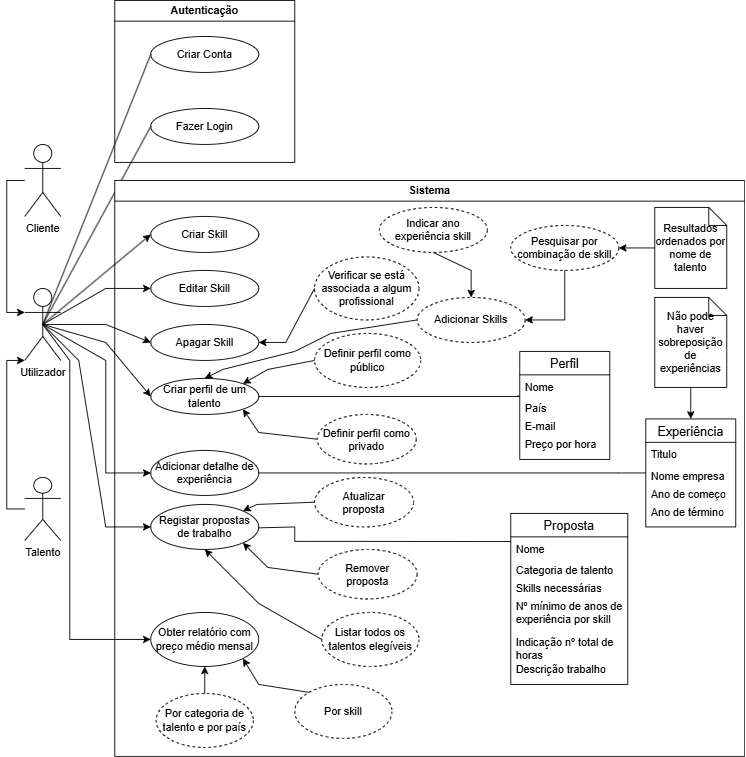
\includegraphics[width=1\linewidth]{imagens/casosdeuso.drawio.png}
    \caption{Modelo de casos de uso}
    \label{fig:1}
\end{figure}

\newpage

\subsection{Modelo de classes}

\begin{figure}[h]
    \centering
    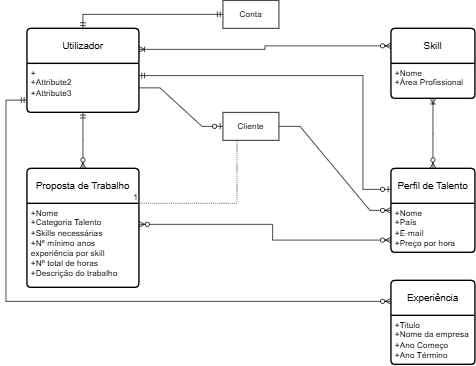
\includegraphics[width=1\linewidth]{imagens/ModelodeClasses.drawio.png}
    \caption{Modelo de classes}
    \label{fig:2}
\end{figure}